\documentclass[landscape,a0paper,fontscale=0.285]{poster}

\usepackage{graphicx}

\usepackage{amsmath}
\usepackage{amssymb}

\usepackage{booktabs}
\usepackage{enumitem}
\usepackage{palatino}
\usepackage[font=small,labelfont=bf]{caption}

\usepackage{multicol}
\setlength{\columnsep}{1.5em}
\setlength{\columnseprule}{0mm}

\usepackage{tikz}
\usetikzlibrary{shapes,arrows}

\newcommand{\compresslist}{
\setlength{\itemsep}{1pt}
\setlength{\parskip}{0pt}
\setlength{\parsep}{0pt}
}

\definecolor{lightblue}{rgb}{0.145,0.6666,1}

\begin{document}

\begin{poster}
{
headerborder=closed,
colspacing=1em,
bgColorOne=white,
bgColorTwo=white,
borderColor=lightblue,
headerColorOne=black,
headerColorTwo=lightblue,
headerFontColor=white,
boxColorOne=white,
textborder=roundedleft,
eyecatcher=true,
headerheight=0.1\textheight,
headershape=roundedright,
headerfont=\Large\bf\textsc,

linewidth=2pt
}

{
\includegraphics[height=5em, trim={0 0 -3cm 0}]{FAIR}}
{\bf\textsc{Revisiting Classifier Two-Sample Tests}\vspace{0.5em}}
{\textsc{ David Lopez-Paz and Maxime Oquab  \hspace{12pt} }}
{
\includegraphics[height=4em]{logo_inria}}

\headerbox{Problem: two-sample tests}{name=objectives,column=0,row=0}{
Given the two samples
\begin{align*}
  S_P := \{ x_1, \ldots, x_n \} &\sim P^n(X),\\
  S_Q := \{ y_1, \ldots, y_m \} &\sim Q^m(Y), \text{ is $P=Q$?}
\end{align*}

To answer, compute a \emph{test statistic} $\hat{t} :=
\hat{t}(S_P, S_Q)$. Then,
reject the \emph{null hypothesis} $H_0 : P = Q$ if
$$\hat{p} = P(T \geq \hat{t} \,|\, H_0) < \alpha = 0.05,$$
to prefer the \emph{alternative hypothesis} $H_1 : P\neq Q$.
}

\headerbox{State-of-the-art: MMD}{name=sota,below=objectives,column=0,row=0}{

The Maximum Mean Discrepancy (MMD) \cite{gretton2012kernel}:
\begin{equation*}
  \hat{t} = \text{MMD}^2(S_P, S_Q) = \| \mu_k(S_P) - \mu_k(S_Q) \|_{\mathcal{H}_k}^2,
\end{equation*}

where
\begin{equation*}
  \mu_k(S) = \frac{1}{|S|} \sum_{x \in S} k(x, \cdot)
\end{equation*}

is the kernel mean embedding associated to a \emph{fixed test representation}
$k(x, \cdot)$.  {\color{red}But, what about learning the test representation
from data?}
}

\headerbox{Contribution: C2ST}{name=c2st,below=sota,column=0,row=0}{
\begin{enumerate}\compresslist
    \item Construct the dataset :
    \begin{equation*}
      \mathcal{D} = \{(x_i, 0)\}_{i=1}^n \cup \{(y_i, 1)\}_{i=1}^n =: \{(z_i, l_i)\}_{i=1}^{2n}.
    \end{equation*}

    \item Split $\mathcal{D}$ into two random halves $\mathcal{D}_\text{tr}$
    and $\mathcal{D}_\text{te}$.

    \item Train a classifier $f : \mathcal{X} \to [0,1]$ on
    $\mathcal{D}_\text{tr}$.

    \item Test $f$ the on $\mathcal{D}_te$ to obtain our \emph{C2ST statistic}:
    \begin{equation}\label{eq:stat}
      \hat{t} = \frac{1}{n_\text{te}} \sum_{(z_i,l_i) \in \mathcal{D}_\text{te}}
      \mathbb{I}\left[ \mathbb{I}\left(f(z_i) > \frac{1}{2}\right) = l_i \right]
    \end{equation}
\end{enumerate}

\vspace{1ex}
}

\headerbox{C2ST Asymptotic Distrib.}{name=distribs,column=1,row=0}{

Each term $\mathbb{I}\left[ \mathbb{I}(f(z_i) > 1/2) = l_i\right]$ appearing
in \eqref{eq:stat} is an independent $\text{Bernoulli}(p_i)$.

\begin{enumerate}\compresslist
  \item \textbf{Null hypothesis} $H_0 : P = Q$,
  \begin{itemize}
    \item the classification is impossible,
    \item $n_\text{te} \hat{t} \sim \text{Binomial}(n_\text{te},p=\frac{1}{2})$.
    \item $n_\text{te} \approx \mathcal{N}(\frac{1}{2}, \frac{1}{4 n_\text{te}})$.
  \end{itemize}
  \item \textbf{Alternative hypothesis} $H_1 : P \neq Q$,
  \begin{itemize}
    \item $\mathbb{I}\left[ \mathbb{I}(f(z_i) > 1/2) = l_i\right]$ with prob. $p_i$,
    \item $n_{\text{te}} \hat{t} \sim \text{PoissonBinomial} ((p_i)_i)$,
    \item $n_{\text{te}} \approx \text{Binomial}(n,\bar{p})$, \newline with
    $\bar{p} = \frac{1}{n}\sum_{i=1}^n p_i$ \cite{Ehm91}.
    \item $n_{\text{te}} \approx \mathcal{N}(\bar{p},
    \frac{\bar{p}(1-\bar{p})}{n_\text{te}})$ (CLT).
   \end{itemize}
\end{enumerate}
}

\headerbox{C2ST Power (Synthetic data)}{name=results,column=2,span=1,row=0}{

\begin{center}
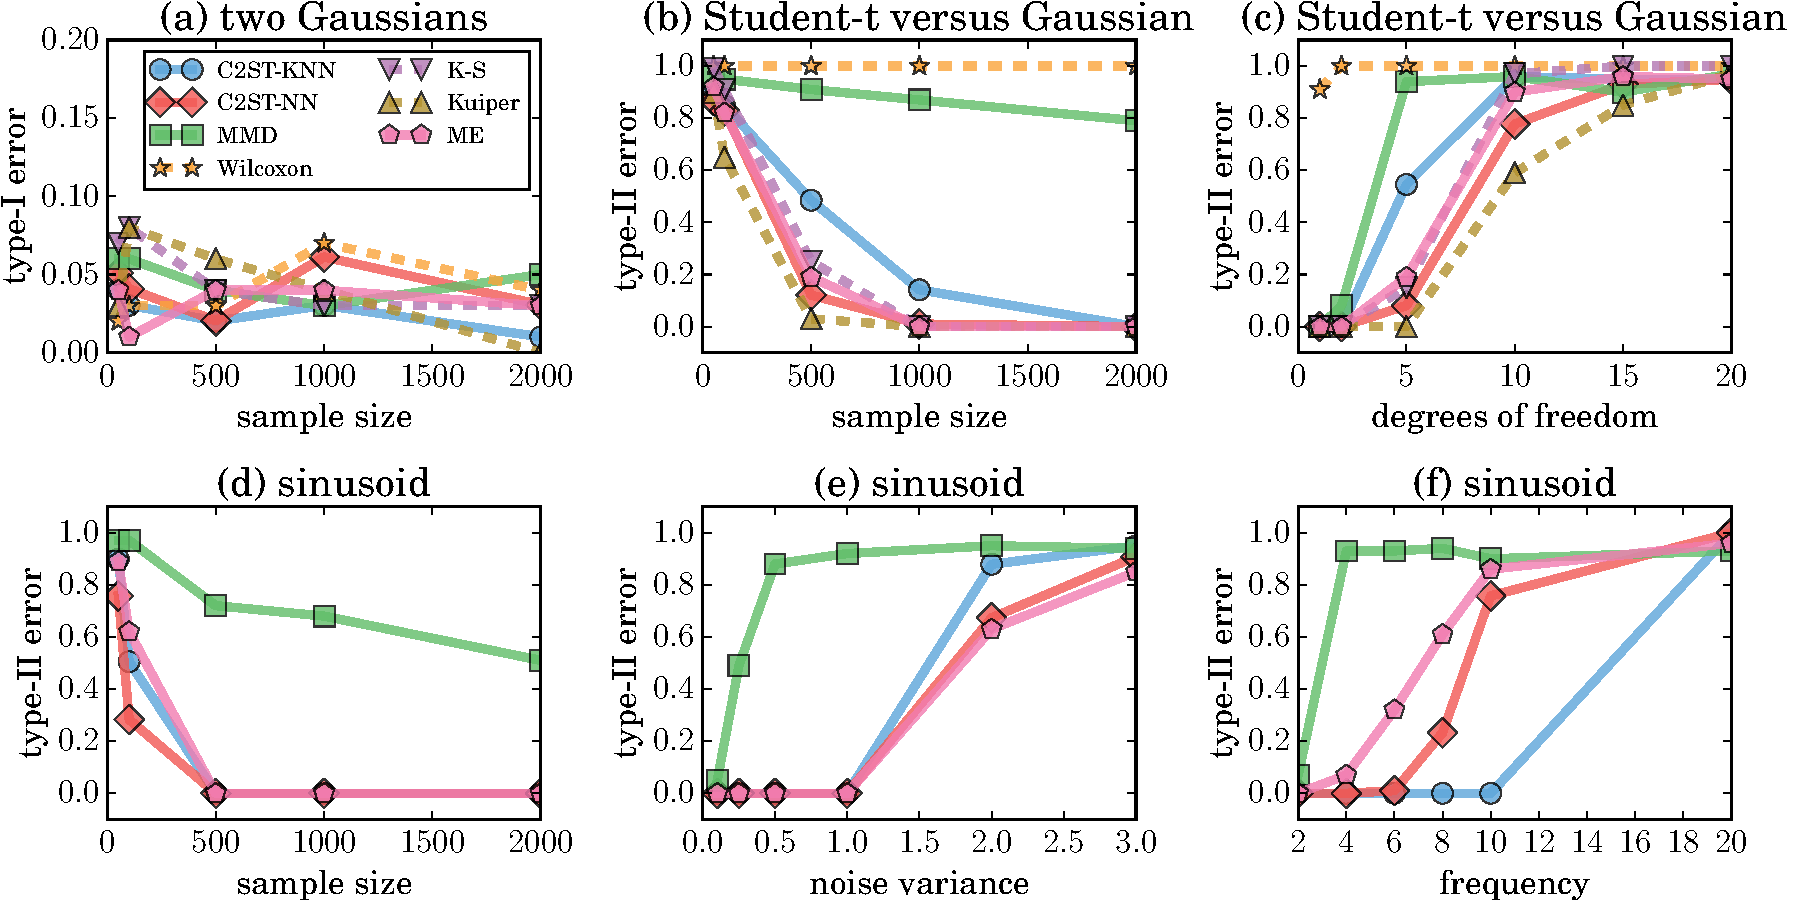
\includegraphics[width=\textwidth]{../figures/synthetic_results.pdf}
\end{center}
\vspace{-3ex}
\captionof{figure}{Type I II errors for synthetic experiments.}
\vspace{1ex}

}
\def\bla{0.12}
\headerbox{C2ST Interpretability}{name=interpretability,column=3,span=1,row=0, bottomaligned=results}{
\begin{multicols}{2}
  \begin{center}
    
\includegraphics[width=\bla\textwidth]{../figures/AM05HAS}
    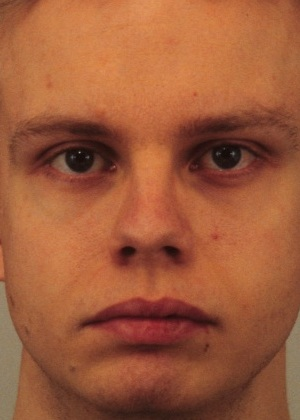
\includegraphics[width=\bla\textwidth]{../figures/AM05NES}
    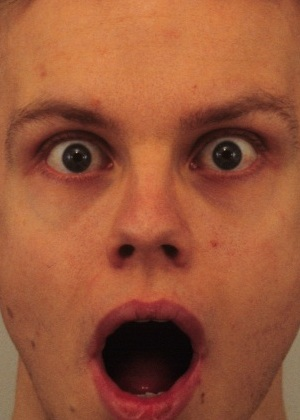
\includegraphics[width=\bla\textwidth]{../figures/AM05SUS}\\
    
\includegraphics[width=\bla\textwidth]{../figures/AM05AFS}
    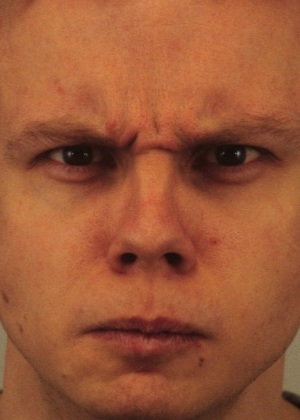
\includegraphics[width=\bla\textwidth]{../figures/AM05ANS}
    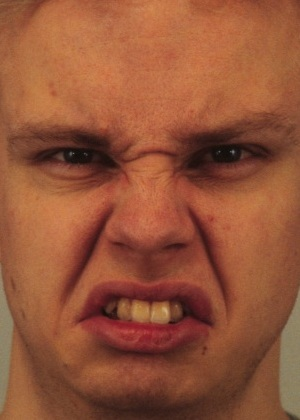
\includegraphics[width=\bla\textwidth]{../figures/AM05DIS}\\
    
\includegraphics[width=\bla\textwidth]{../figures/faces_diff_happy}
    
\includegraphics[width=\bla\textwidth]{../figures/faces_diff_angry}
    
\includegraphics[width=\bla\textwidth]{../figures/faces_diff_diff}
  \end{center}
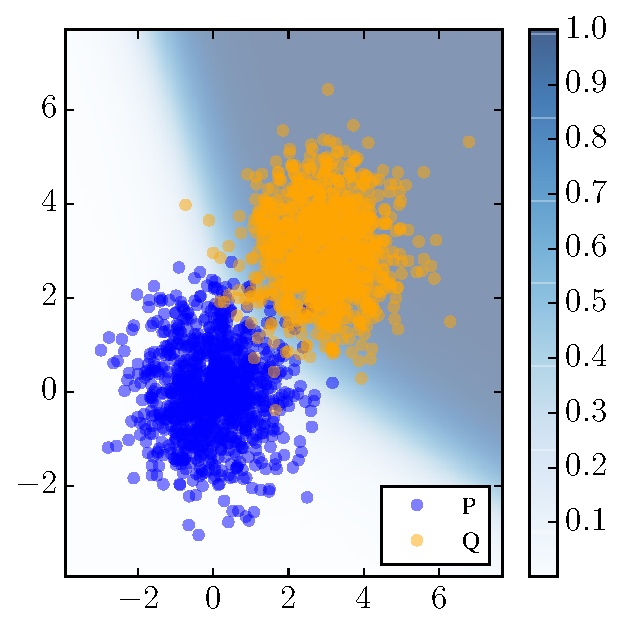
\includegraphics[width=0.48\textwidth, trim={4ex 0 0 0}, clip ]{../figures/interpret_1.pdf}

\end{multicols}
\vspace{-3ex}
\captionof{figure}{Interpretability of C2ST (color is $p(l=1|z)$).}
}

\headerbox{References}{name=references,column=0, span=2,below=c2st}{
\begin{multicols}{3}
\renewcommand{\section}[2]{\vskip 0.05em}
\nocite{*}
\small{
\bibliographystyle{unsrt}
\bibliography{sample}
}
\end{multicols}
}

\headerbox{C2ST Power (real data)}{name=news,column=2,span=2,row=0,below=results,below=results}{

\begin{center}
  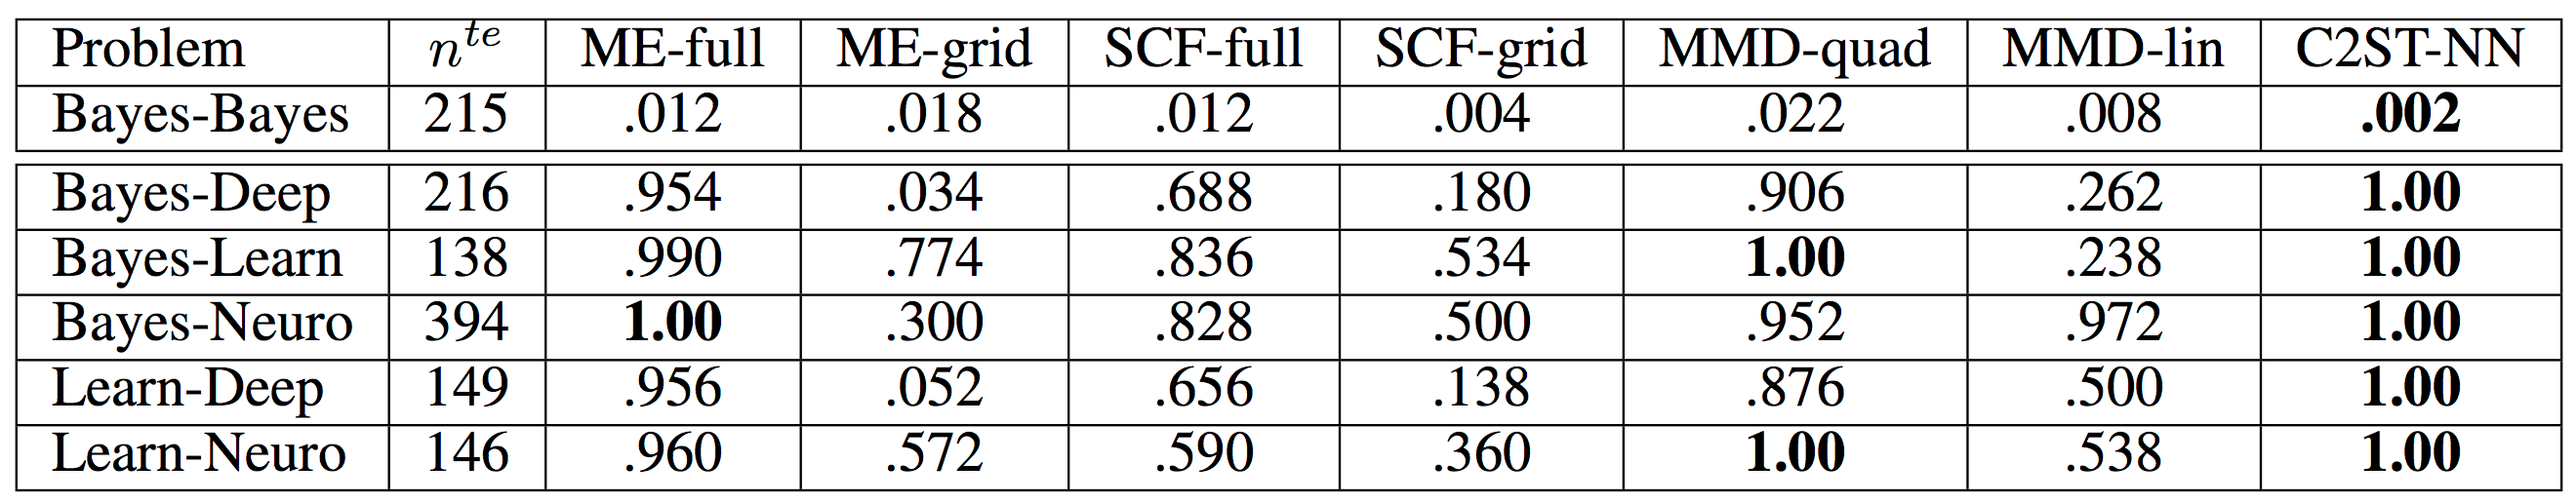
\includegraphics[width=0.7\textwidth]{extra_1}
\end{center}
\vspace{-3ex}
\captionof{figure}{Type-I errors (first row) and powers (rest of rows) in
distinguishing NIPS papers categories.}

\begin{center}
  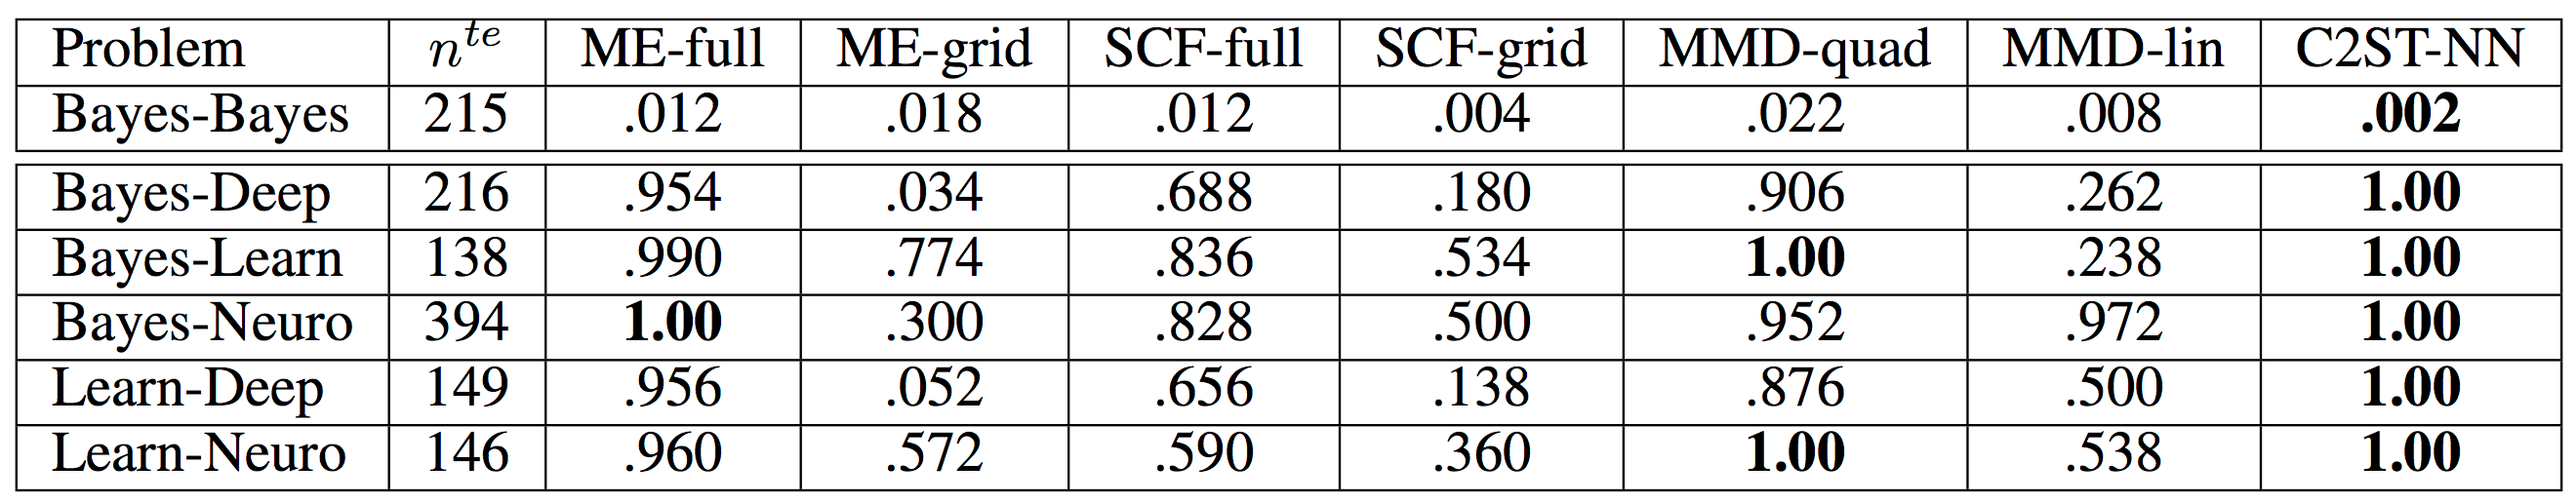
\includegraphics[width=0.7\textwidth]{extra_1}
\end{center}
\vspace{-3ex}
\captionof{figure}{Type-I errors (first row) and powers (second row) in
distinguishing facial expressions.}
}


\headerbox{Evaluating the quality of GANs with
C2ST}{name=conclusion,column=2,span=2,row=0,below=news}{

\begin{center}
  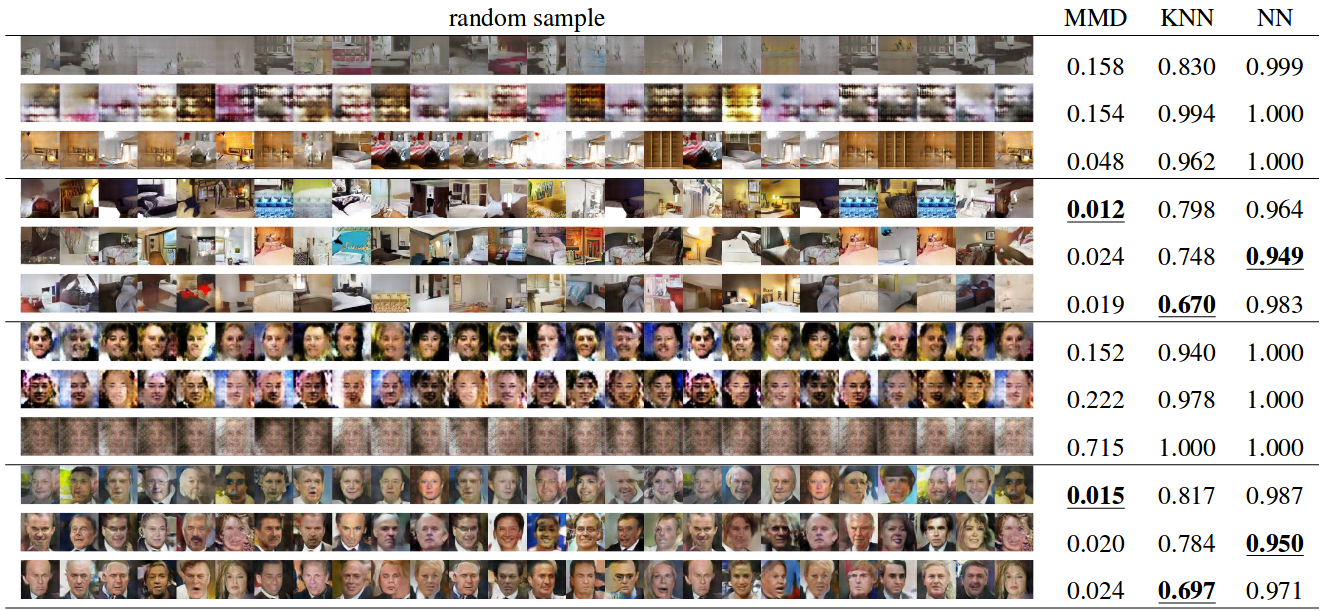
\includegraphics[width=0.8\textwidth]{figtablegans}
\end{center}
\vspace{-3ex}
\captionof{figure}{Results on GAN evaluation. Lower test statistics $\equiv$
better GAN. }
}

\headerbox{Testing
power}{name=results2,column=1,below=distribs,bottomaligned=c2st}{

The \emph{significance level} $\alpha$
upper-bounds the \emph{type-I error (probability rejecting a true
$H_0$)}. Given $\alpha$, we choose the test with maximum
power, or minimal \emph{type-II error (probability of
accepting a false $H_0$)}.\\

Assuming that we can compute the empirical risk minimizer $f^\star$, and that
$f^\star$ has expected risk:
\begin{itemize}\compresslist
  \item $H_0: t = \frac{1}{2}$ under $H_0 : P=Q$,
  \item $H_1: t = \frac{1}{2} + \epsilon$ under $H_1 : P\neq Q$,
\end{itemize}

where $\epsilon \in (0, \frac{1}{2})$ is also known as the \emph{effect size}.\\

The approximate power \emph{(probability of correctly rejecting a false null
hypothesis)} of the C2ST \eqref{eq:stat} is $$\Phi\left(
\frac{\epsilon\sqrt{n_\text{te}}-\Phi^{-1}(1-\alpha)/2}{\sqrt{\frac{1}{4}-\epsilon^2}}\right)$$
}

\end{poster}

\end{document}
